\documentclass[handout]{beamer}
\usetheme{Madrid}
\usepackage{pdfpages}
\usepackage[utf8x]{inputenc}
\usepackage{url}
\usepackage{graphicx}
\usepackage{graphics}
\usepackage{adjustbox}
\usepackage{ragged2e}
\usepackage{amsmath, amssymb}
\usepackage{verbatim}
\usepackage{soul}
\usepackage{textpos}
\usepackage{xcolor}
\usepackage{tcolorbox}
\usepackage{lmodern,textcomp}
 \setbeamertemplate{enumerate items}[default]
 \setbeamertemplate{itemize items}[circle]
 \setbeamertemplate{frametitle continuation}{}
\setbeamertemplate{section in toc}[circle]
\setbeamertemplate{subsection in toc}[circle]

\usepackage{tabulary, booktabs}

\usepackage{hyperref}
\hypersetup{
    colorlinks=cyan,
    linkcolor=true,
    filecolor=cyan,      
    urlcolor=cyan,
}

\beamertemplatenavigationsymbolsempty

%%%%%%%%%%%%%%%Color%%%%%%%%%%%%%%%
\definecolor{KIPlum}{HTML}{880052}
\definecolor{box}{RGB}{250, 117, 144}
\usecolortheme[named=KIPlum]{structure}

%%%%%%%%%%%%%%%Bibliography setting%%%%%%%%%%%%%%%
\usepackage[numbers,comma,sort&compress]{natbib}
\makeatletter
\renewcommand{\@biblabel}[1]{#1.} %remove brackets from the ref list
\makeatother




%%%%%%%%%%%%%%%Title page%%%%%%%%%%%%%%%

\title[Applied Epi I: Summary Statistics and Graphs]{Applied Epidemiology I: Summary Statistics and Graphs}
\date{\today}
\author[Enoch Yi-Tung Chen]{Enoch Yi-Tung Chen}
\institute[MEB]{Department of Medical Epidemiology and Biostatistics, Karolinska Insitutet}

%%%%%%%%%%%%%%\begin{document}%%%%%%%%%%%%%%%%

\begin{document}

\begin{frame}
\maketitle 
\end{frame}

%%%%%%%%%%%%%%Ack%%%%%%%%%%%%%%%%
\begin{frame}{Acknowledgements}
This course material is based on my learning from \href{https://staff.ki.se/people/analam}{Anastasia Lam}'s teachings in last year's Applied Epidemiology I lab sessions, and readings from \textit{Epidemiology} by Gordis \cite{Gordis2014}, \textit{A First Course in Probability and Statistics} by Goldsman and Goldsman \cite{Goldsman2020}, \textit{Principles of Biostatistics} by Pagano and Gauvreau \cite{Pagano2000}, and \textit{Biostatistics I} by Gabriel and Frumento \cite{Gabriel2020}. 

I especially want to thank Marlene Stratmann for reviewing the slides and Prof. Paul Dickman for providing me with suggestions to improving the teaching.

\end{frame}



%%%%%%%%%%%%%%Outline%%%%%%%%%%%%%%%%
\section*{Outline}
\begin{frame}{Outline}
          \tableofcontents
\end{frame}

%%%%
\section{Summary statistics}
\subsection{Bad example}
\begin{frame}{\secname: \subsecname}
What is the problem here? \\
\begin{center}
	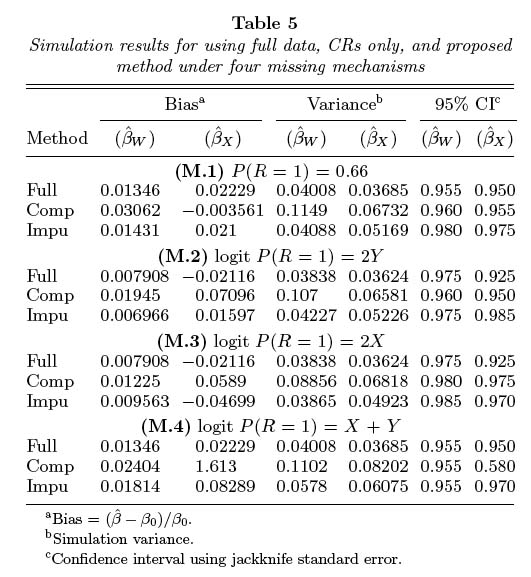
\includegraphics[scale=0.4]{images/paik_tab5}
\end{center}

	
\end{frame}


\subsection{Measures of Central Tendency: mean, median, mode}
\begin{frame}[fragile]{{\secname: \\ \subsecname}}	
\begin{itemize}
	\item<1|handout:1-> Mean: the sum of the values of a variable and dividing
by number of the observations
	\item<2|handout:2->  Median: the middle (the 50th centile) observation
	\item<3|handout:3->  Mode: the value that occurs most frequently
	\item<4|handout:4>  []
\scriptsize
\begin{verbatim}

. tabstat age // will only give you mean

    variable |      mean
-------------+----------
         age |  56.41176
------------------------

. tabstat age, s(count mean median) // s stands for statistics
    variable |         N      mean       p50
-------------+------------------------------
         age |        34  56.41176        56
--------------------------------------------
	
\end{verbatim}

\end{itemize}
\end{frame}

%%%%
\subsection{Measures of Dispersion: range, IQR, variance, standard deviation}
\begin{frame}[fragile]{{\secname: \subsecname}}	
\begin{itemize}
	\item<1|handout:1-> Range: the difference between the maximum and the minimum 
	\item<2|handout:2-> Interquartile range: the absolute difference between the 25th percentile of the observations and the 75th.
	\item<3|handout:3-> Variance, standard deviation (sd): a measure of spread of the data
	\item[]<4|handout:4>
\footnotesize
	\begin{displaymath}
s^{2} = \widehat{Var}(x)=\frac{1}{n-1} \sum_{i=1}^{n}\left(x_{i}-\bar{x}\right)^{2}
\end{displaymath}

\scriptsize
\begin{verbatim}


. tabstat age, s(count range min max iqr var sd)

    variable |         N     range       min       max
-------------+----------------------------------------
         age |        34        20        47        67
------------------------------------------------------

    variable |       iqr  variance        sd
-------------+------------------------------
         age |        10  36.12834  6.010686
--------------------------------------------
\end{verbatim}

\end{itemize}
\end{frame}

%%%%
\section{Graphs}
\subsection{Bad examples}
\begin{frame}[allowframebreaks]{\secname: \subsecname}
	Graphs can say more than texts! But it depends..... \\
	Sometimes less is more. \\
	\begin{center}
			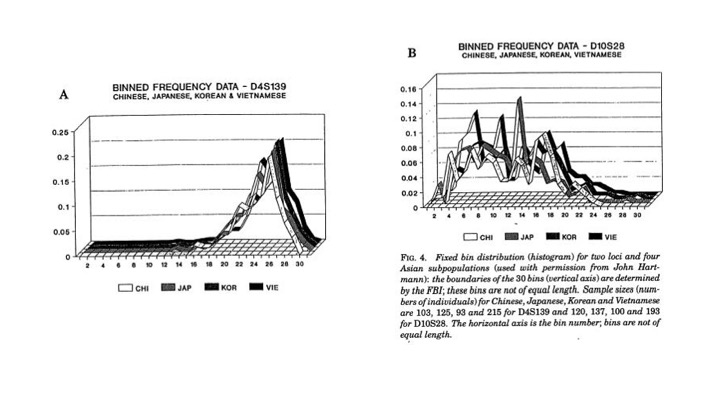
\includegraphics[scale=0.3]{images/Example2}

	\end{center}

	
	\framebreak
	
	Too fancy? \\
	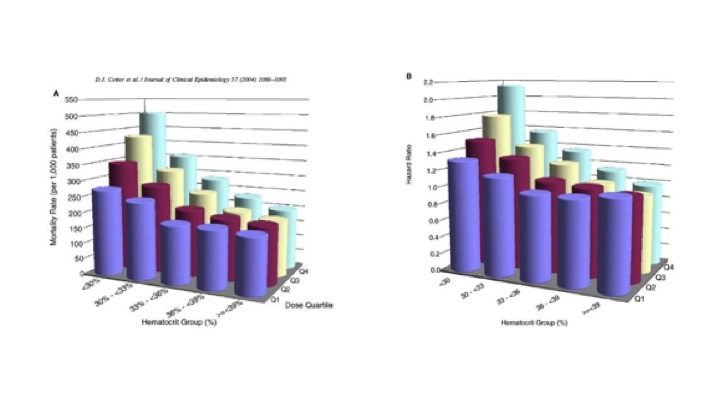
\includegraphics[scale=0.3]{images/Example1}
	
	\framebreak
	
		Insufficient info?

	\begin{center}
			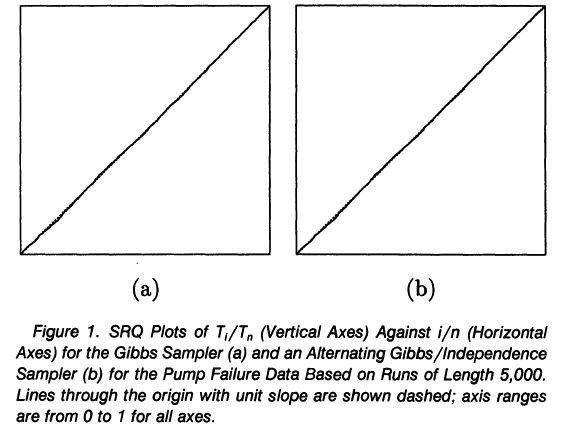
\includegraphics[scale=0.5]{images/Example3}
	\end{center}
	
	\framebreak 
	
	Sometimes there is no right nor wrong, it just depends on your interest.
		\begin{center}
				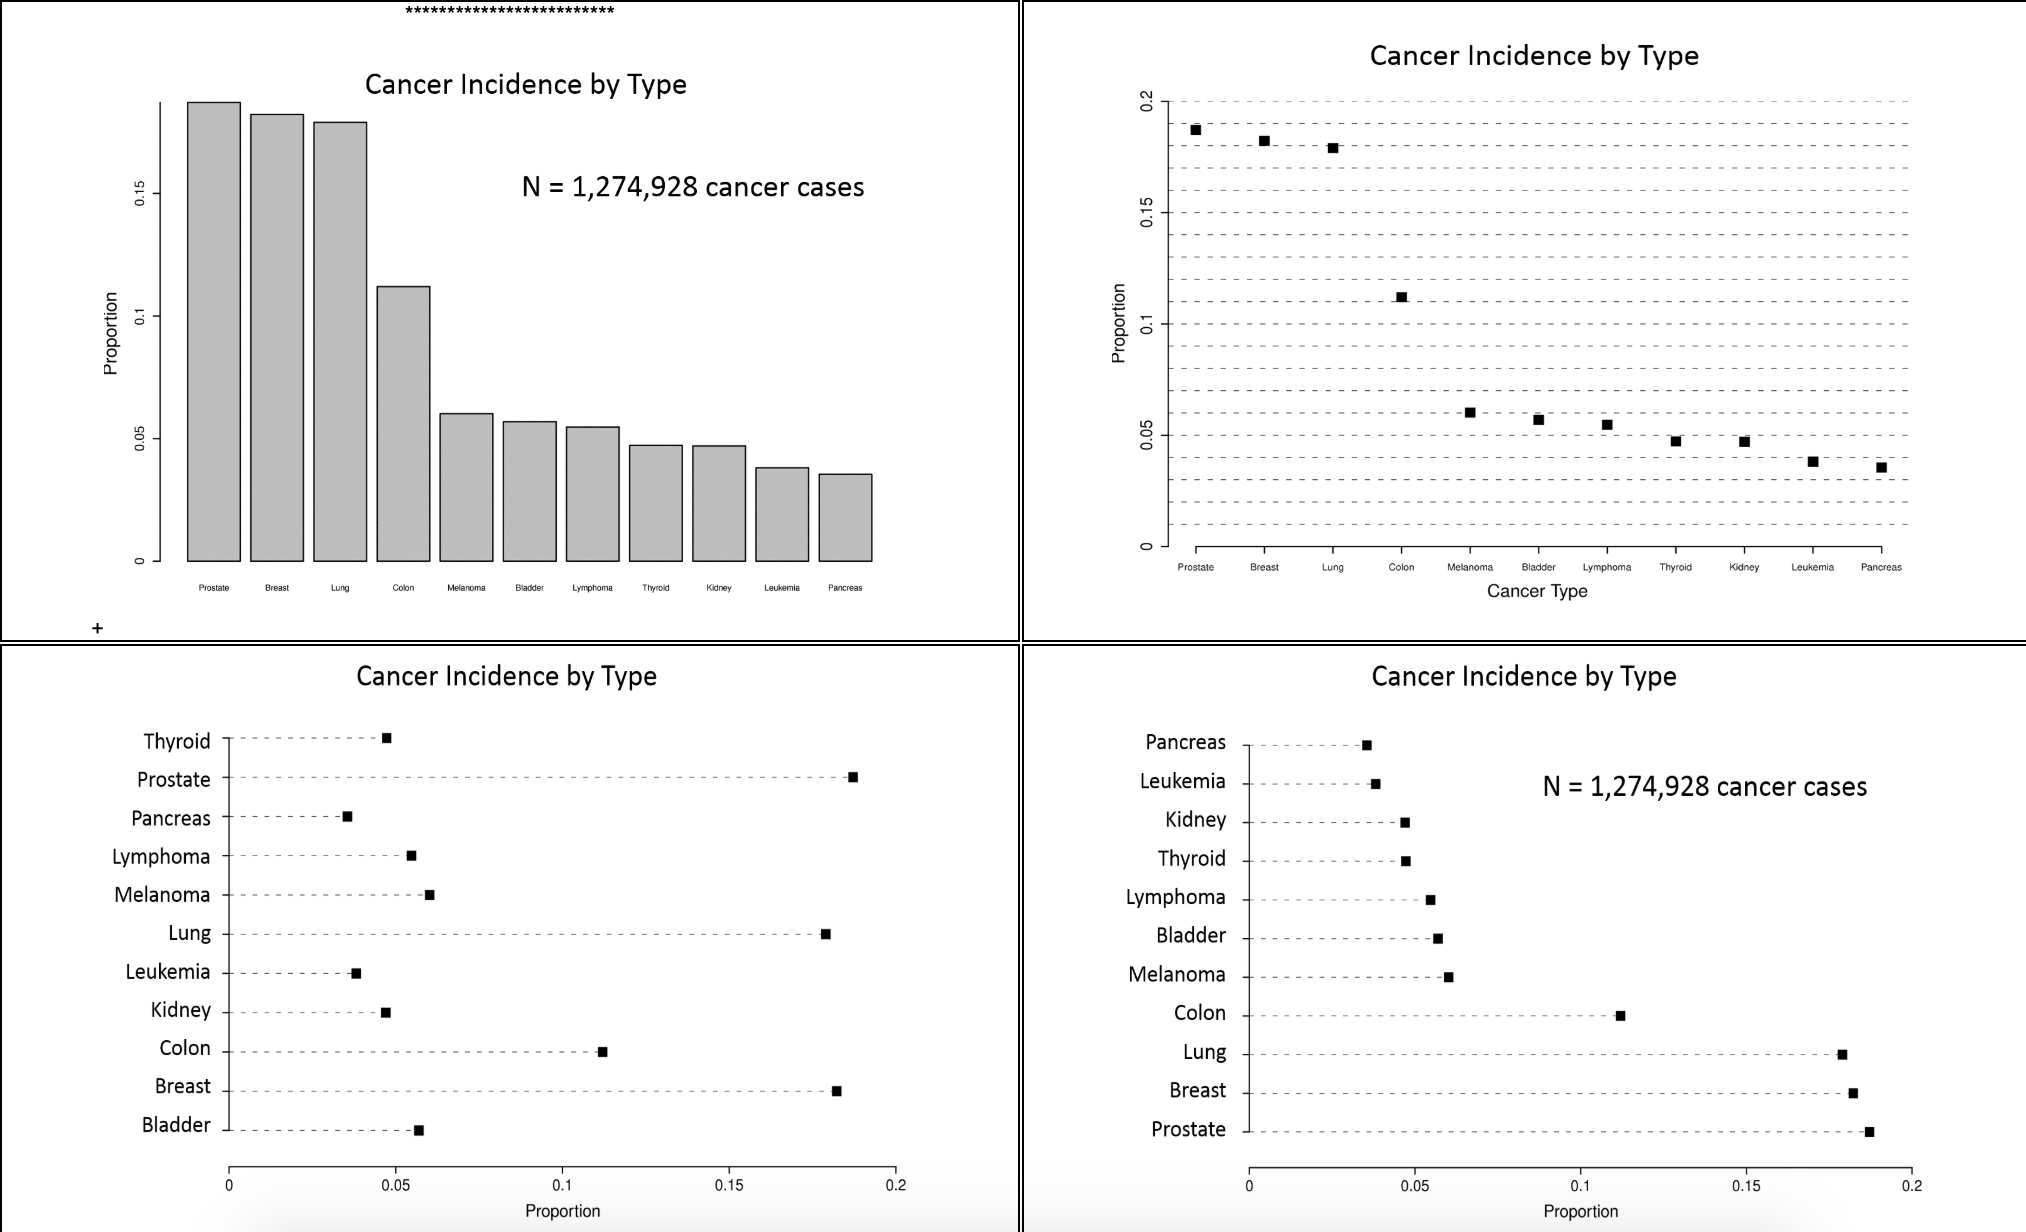
\includegraphics[scale=0.3]{images/Cancer_incidence}
		\end{center}

\end{frame}

%%
\subsection{Learning from errors}
\begin{frame}[fragile]{\secname: \subsecname}
Which part went wrong here? \\
Hint: something was missed in the code.

\small
\begin{verbatim}
twoway connected prop diagyear, ///
subtitle("Proportion of HL patients") ///
ytitle(Proportion splenectomy) ///
xlabel(1973(2)1995) 	
\end{verbatim}
\begin{center}
	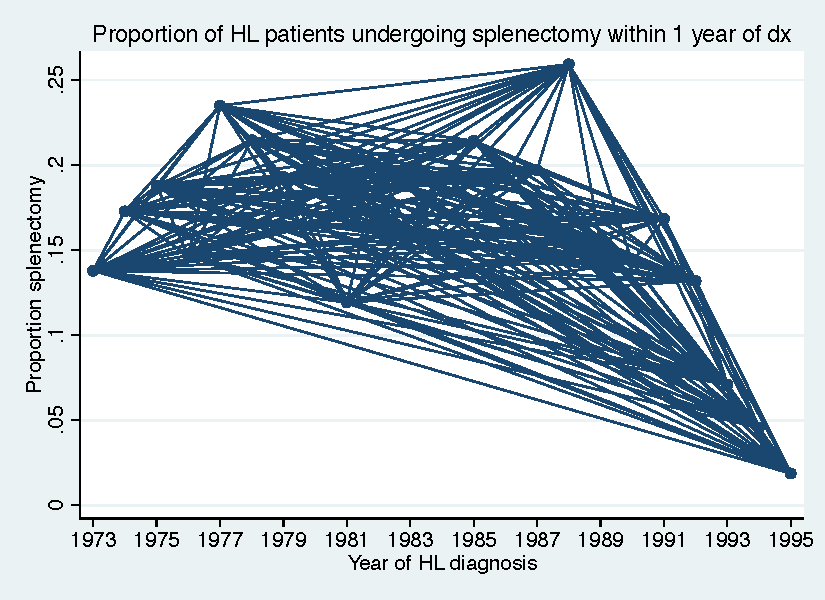
\includegraphics[scale=0.4]{images/nosort}
\end{center}
\end{frame}

\begin{frame}[fragile]{\secname: \subsecname}
It makes such a big difference if you missed \verb|sort|!

\small
\begin{verbatim}
twoway connected prop diagyear, ///
subtitle("Proportion of HL patients") ///
ytitle(Proportion splenectomy) ///
xlabel(1973(2)1995) ///
sort	
\end{verbatim}
\begin{center}
	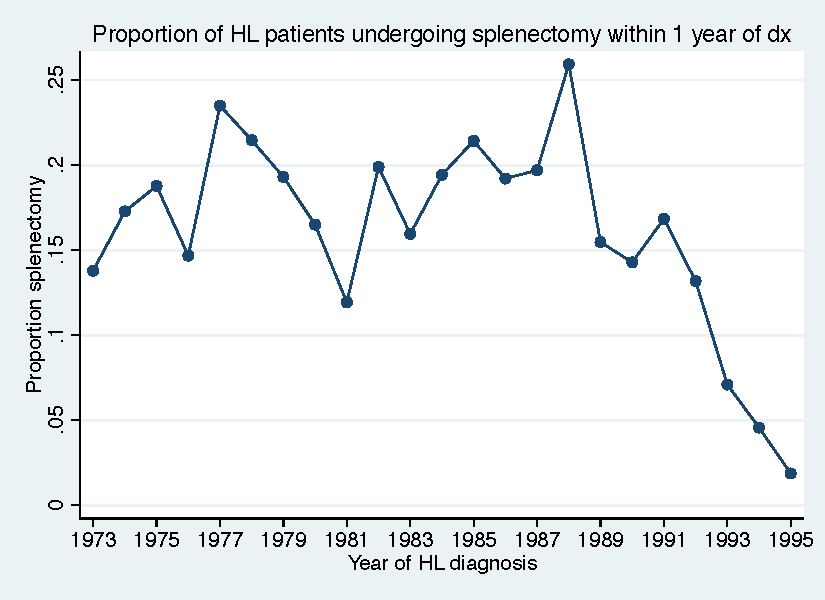
\includegraphics[scale=0.4]{images/sort}
\end{center}

\end{frame}
%%
\subsection{Histogram}
\begin{frame}[fragile]{\secname: \subsecname}
Histogram depicts the distribution of data, where x-axis is usually a continuous variable.
\begin{verbatim}
hist lexp, title("Histogram of Life Expectancy") ///
           xtitle(Age (years)) width(1) /// By each age
           graphregion(color(white)) //	
\end{verbatim}

\begin{center}
	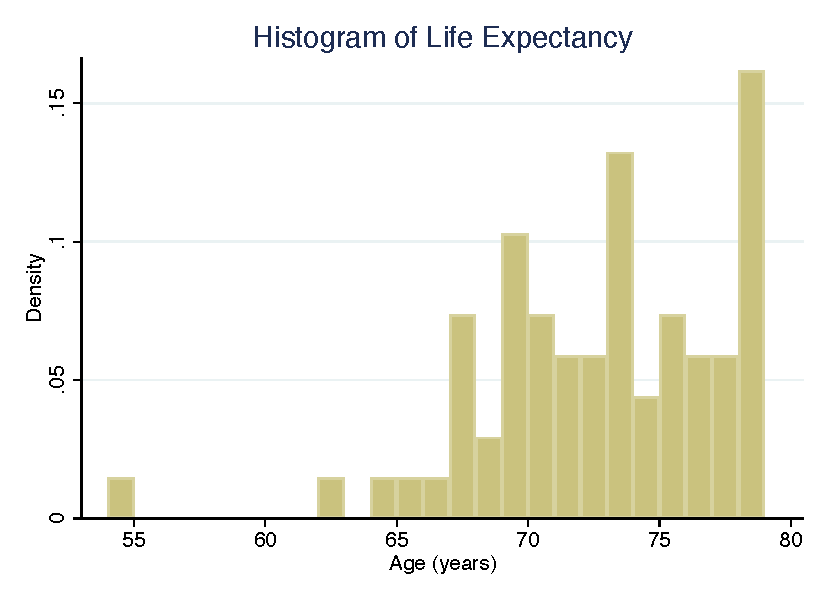
\includegraphics[scale=0.5]{images/hist}
\end{center}

\end{frame}

%%%
\subsection{Bar chart}
\begin{frame}[fragile]{\secname: \subsecname}
Bar chart shows the distribution of discrete (categorical) data.
\begin{verbatim}
graph bar (count), over(region) ///
                   title("Bar chart of Regions") ///
                   graphregion(color(white)) //
\end{verbatim}

\begin{center}
	
\includegraphics[scale=0.5]{images/bar}
\end{center}
\end{frame}

%%%
\subsection{Scatter plot}
\begin{frame}[fragile]{\secname: \subsecname}
Scatter plot demonstrates the relationship between two continuous variables.
\begin{verbatim}
twoway scatter lexp gnppc, graphregion(color(white)) 
\end{verbatim}

\begin{center}
	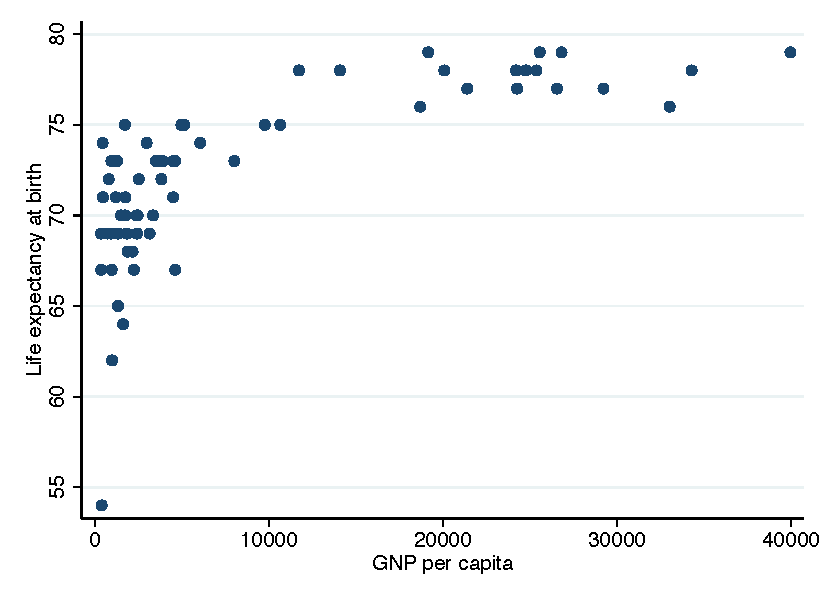
\includegraphics[scale=0.5]{images/scatter}
\end{center}
\end{frame}

%%%
\subsection{Box plot}
\begin{frame}[fragile]{\secname: \subsecname}
Box plot summarises the distribution of the data, with the 25th, 50th,
and 75th percentile and 1.5 IQR.
\begin{verbatim}
graph box lexp, over (region) ///
                graphregion(color(white))\end{verbatim}

\begin{center}
	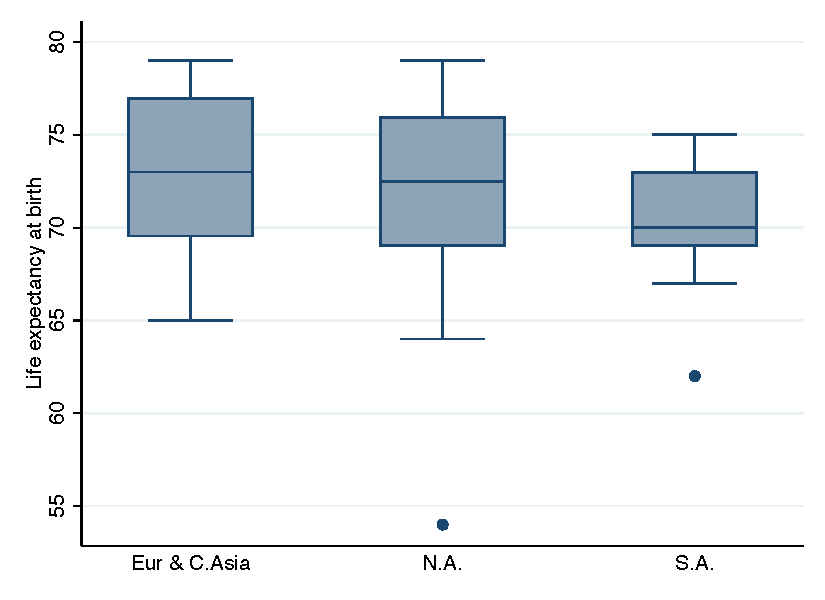
\includegraphics[scale=0.5]{images/box}
\end{center}
\end{frame}
%%%
\subsection{Line graph}
\begin{frame}[fragile]{\secname: \subsecname}
Line graph functions similarly as scatter plots, with time as x-axis usually.
\small
\begin{verbatim}
sysuse uslifeexp, clear
twoway line le year, title("Life expectancy at birth by year, USA") ///
       graphregion(color(white)) }
\end{verbatim}
\begin{center}
	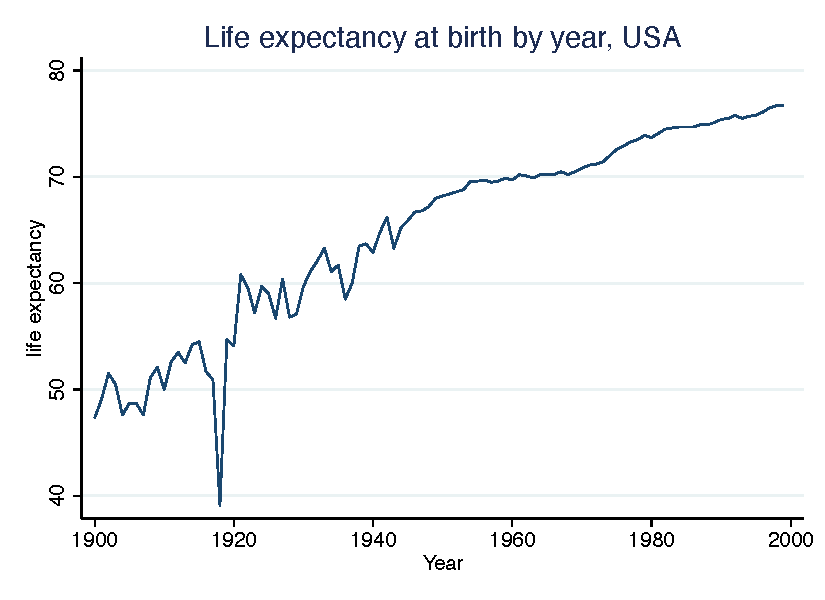
\includegraphics[scale=0.5]{images/line}
\end{center}
\end{frame}

%%%

%%%
\subsection{Stratification}
\begin{frame}[fragile]{\secname: \subsecname}
Data is already in separate columns. Or using \verb|by()|. \\
Hint: \verb|by()| is often used in individual-level data. \\
Btw, why did I use one solid line and the other dash line here?
\begin{center}
	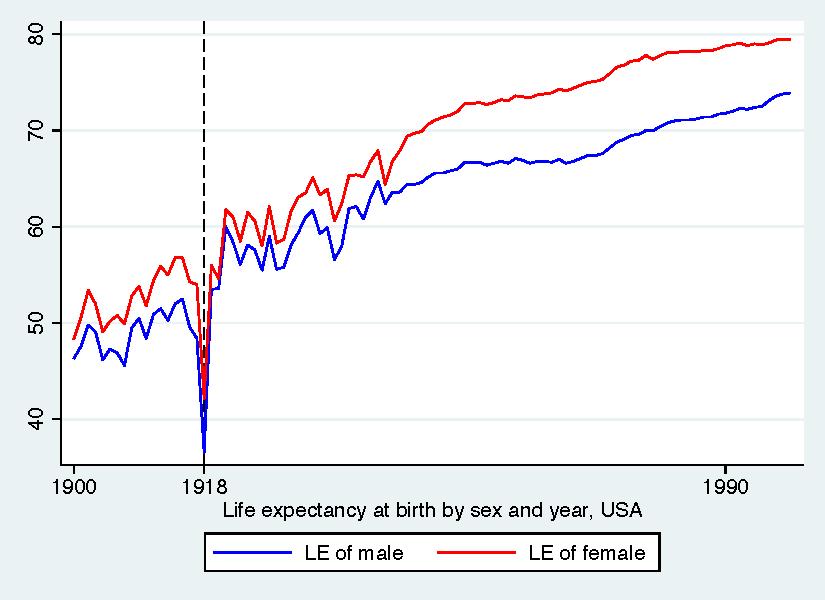
\includegraphics[scale=0.5]{images/stratification}
\end{center}

\end{frame}
%%%
\subsection{Putting graphs together}
\begin{frame}[fragile]{\secname: \subsecname}
\verb|grc1leg2| plays the role in plotting graphs together. \\
Hint: \verb|grc1leg2| is not a default Stata command. See \verb|help grc1leg2| to install it.
\begin{center}
	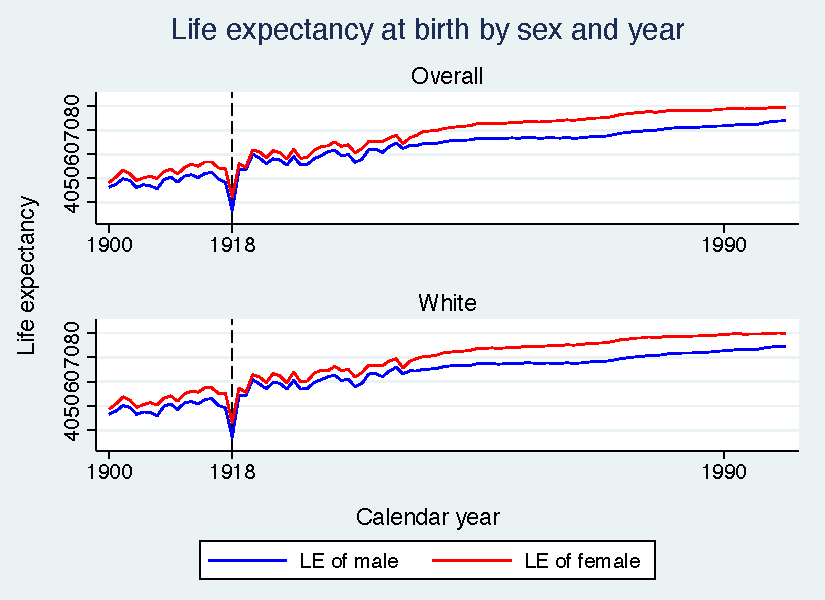
\includegraphics[scale=0.5]{images/grc1leg2}
\end{center}
\end{frame}

%%%
\subsection{Export}
\begin{frame}[fragile]{\secname: \subsecname}
\begin{itemize}
	\item A standard way: 
	\item[] \begin{verbatim}
graph export "location" /// assign the location
, as(pdf) name("")	
 \end{verbatim}
	\item An intuitive way: \\
	\begin{center}
	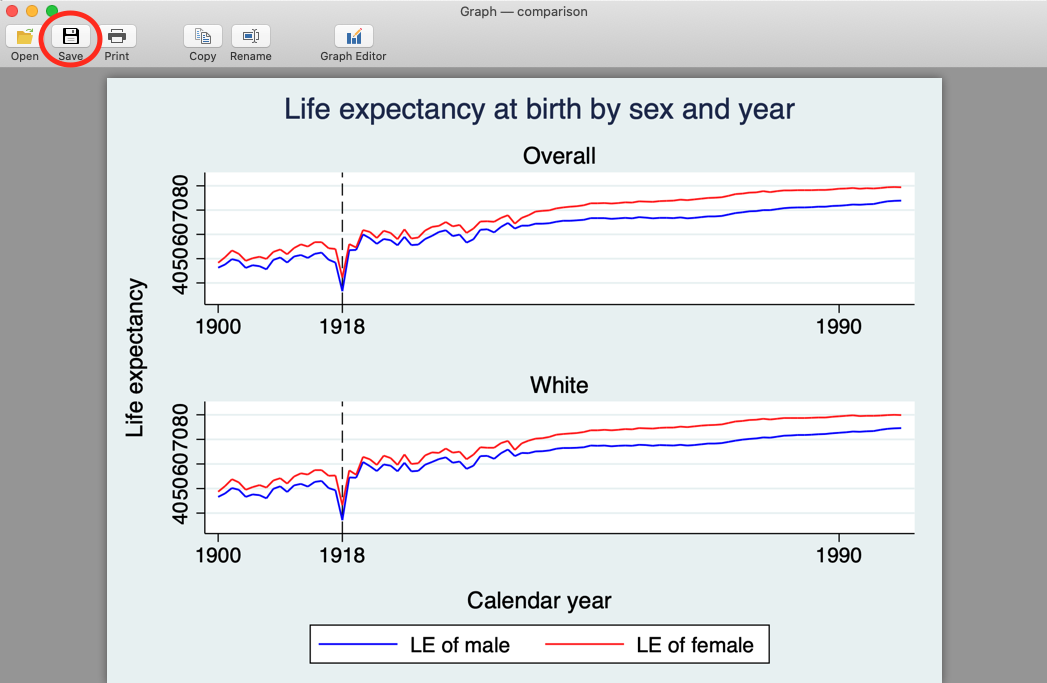
\includegraphics[scale=0.15]{images/export}
\end{center}
\item And then copy and paste the code back to the do-file.
\end{itemize}

\end{frame}

%%
\subsection{Study map}
\begin{frame}{\secname: \subsecname}
Check the webpage: \url{https://extremepresentation.com/tools/}

\begin{center}
	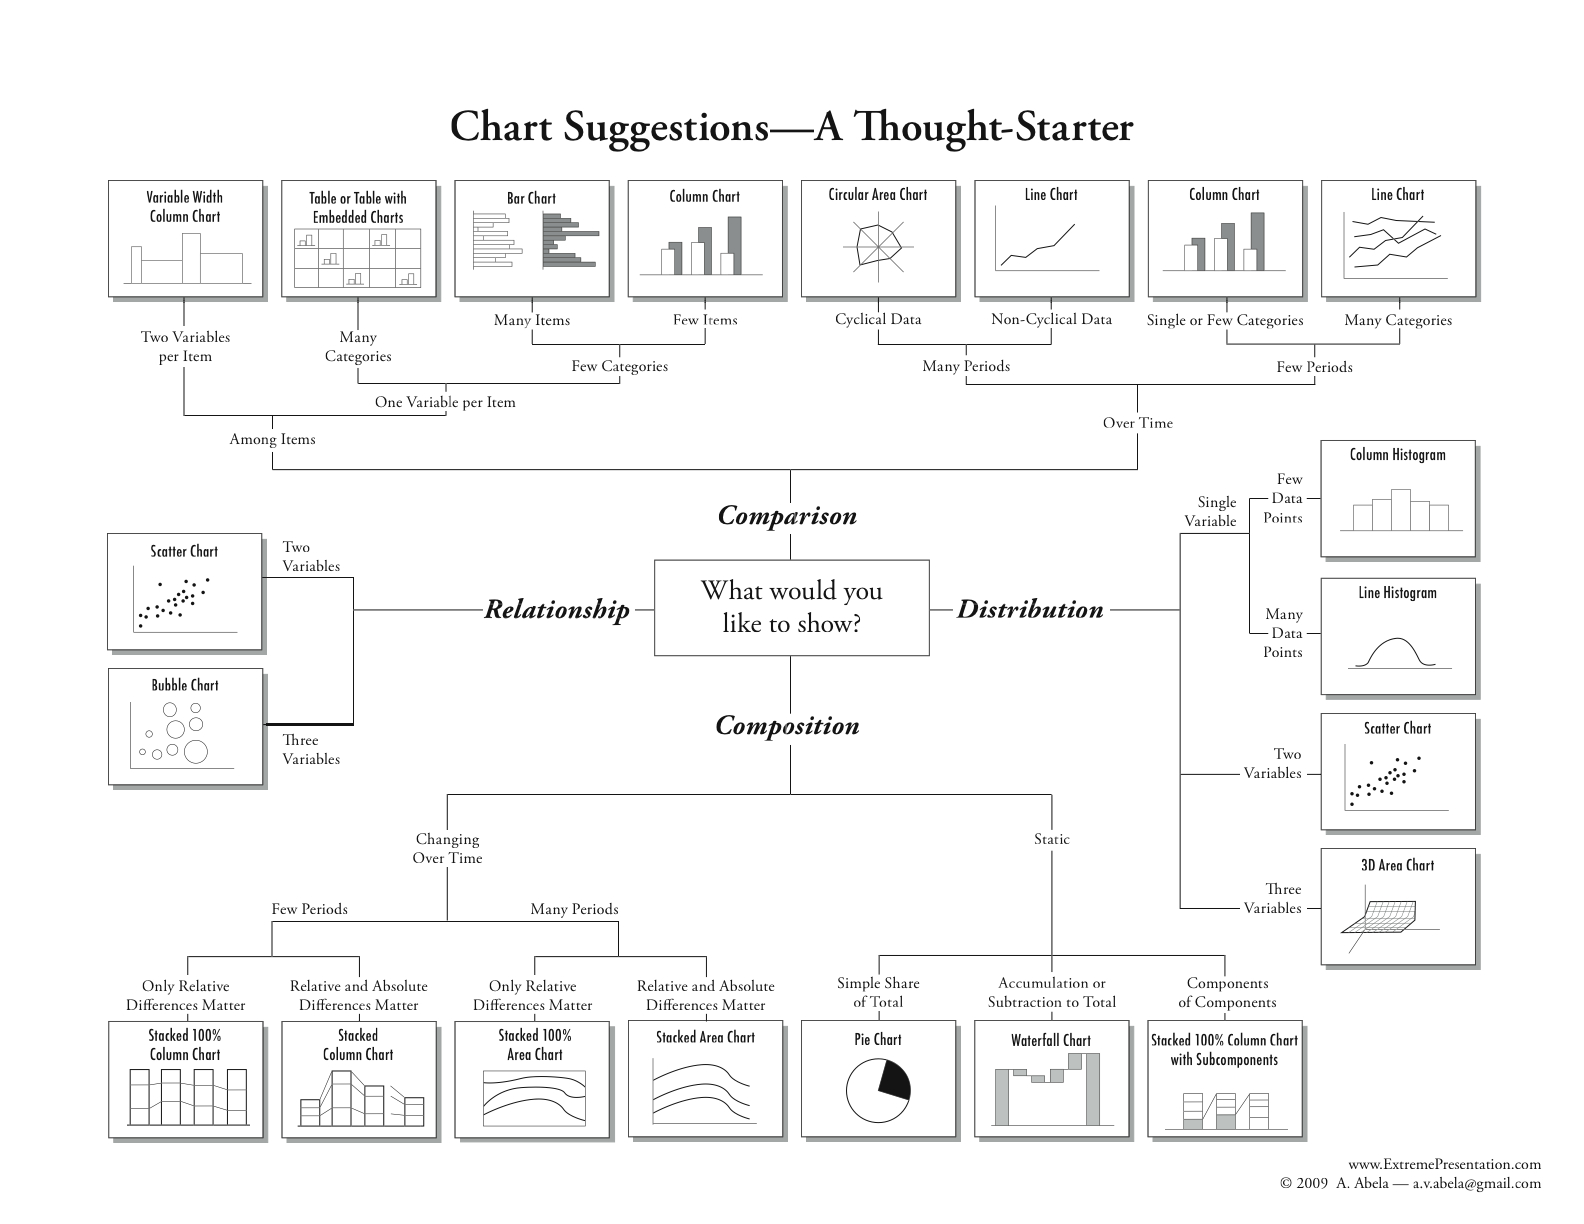
\includegraphics[scale=0.35]{images/chart}
\end{center}

\end{frame}

%%%
\section{References}
\begin{frame}[allowframebreaks,fragile]{\secname}
    \begin{scriptsize}
	\bibliographystyle{../bib/vancouv12}
	\bibliography{../bib/enochref.bib}
    \end{scriptsize}
\end{frame}

\end{document}